\documentclass[german]{spicker}
\usepackage{tabularx}
\usepackage{textcomp}
\usepackage{float}

%\addbibresource{para.bib}

\title{Parallele Rechnerarchitekturen}
\subtitle{Sommersemester 2023}
\university{Fachhochschule Aachen}
\programme{Angewandte Mathematik und Informatik, M. Sc.}
\lecturer{Dr. Marcus Richter, Jochen Kreutz}

\author{Sven Bergmann, Patrick Gustav Blaneck}

\makeindex[intoc]
\makeindex[intoc, name=Beispiele,title=Beispiele]

% Setup for SI units
\sisetup{
  per-mode=fraction,
  fraction-function=\tfrac
}
\DeclareSIUnit{\flops}{FLOPS}
\DeclareSIUnit{\cores}{cores}
\DeclareSIUnit{\cycle}{cycle}
\DeclareSIUnit{\cycles}{cycles}

\begin{document}
\maketitle
\tableofcontents
\disclaimer

\section{Rechnerarchitekturen}\label{sec:rechnerarchitekturen}

\subsection{Einführung}\label{subsec:einfuehrung}

\begin{defi}{Struktur}
    Unter der \emph{Struktur} einer Rechnerarchitektur versteht man die Art der Verknüpfung der verschiedenen Hardwarekomponenten eines Rechner miteinander.

    Sie ist in der Regel \emph{statisch}.
\end{defi}

\begin{defi}{Organisation}
    Die \emph{Organisation} einer Rechnerarchitektur steht für die zeitabhängigen Wechselwirkungen zwischen Komponenten und die Steuerung dieser Komponenten.

    Diese Wechselwirkungen können \emph{dynamisch} sein.
\end{defi}

\begin{defi}{Implementierung}
    Die \emph{Implementierung} einer Rechnerarchitektur bezeichnet die Ausgestaltung einzelner Bausteine.

    Sie gibt die \emph{Größe} eines Systems an.
\end{defi}

\begin{defi}{Leistung}
    \emph{Leistung} beschreibt das nach außen hin sichtbare Systemverhalten.

    Sie gibt die \emph{Geschwindigkeit} eines Systems an.
\end{defi}

\subsection{Von-Neumann-Rechner}\label{subsec:von-neumann-rechner}

\begin{defi}{Von-Neumann-Rechner}
    Der \emph{Von-Neumann-Rechner} besteht aus folgenden Werken:
    \begin{itemize}
        \item \emph{Eingabe- bzw. Ausgabewerk:}
              \begin{itemize}
                  \item Schnittstelle zur Außenwelt
              \end{itemize}
        \item \emph{Leitwerk:}
              \begin{itemize}
                  \item interpretiert Befehle
                  \item steuert Abläufe
              \end{itemize}
        \item \emph{Haupt- bzw. Arbeitsspeicher:}
              \begin{itemize}
                  \item Speicher für Daten \emph{und} Befehle
                  \item unterteilt in Zellen gleicher Größe geteilt, die durch fortlaufende Adressen identifiziert werden
              \end{itemize}
        \item \emph{Rechenwerk:}
              \begin{itemize}
                  \item führt arithmetische und logische Operationen aus
              \end{itemize}
    \end{itemize}

    Die Struktur des Rechners ist unabhängig von der Aufgabe, die er lösen soll.
    Hardware und Software sind voneinander \emph{getrennt}.
\end{defi}

\begin{defi}[Von-Neumann-Rechner]{Struktur}
    TODO
\end{defi}

\begin{defi}[Von-Neumann-Rechner]{Organisation}
    TODO
\end{defi}

\begin{defi}[Von-Neumann-Rechner]{Arbeitsweise}
    Die \emph{Von-Neumann-Architektur} erlaubt nacheinander (\emph{sequentiell}):

    \begin{itemize}
        \item das Lesen eines Befehlscode-Worts oder
        \item das Lesen eines Datenworts oder
        \item das Schreiben eines Datenworts.
    \end{itemize}

    Befehlscode-Lesen und Daten-Lesen und -Schreiben konkurrieren.

    Von der Folge kann durch bedingte und unbedingte Sprungbefehle abgewichen werden, die die Programmfortsetzung an einer anderen Zelle bewirken.

    Die Maschine benutzt Binärcodes, Zahlen werden dual dargestellt.
\end{defi}

\begin{defi}[Von-Neumann-Rechner]{Von-Neumann-Flaschenhals}
    Der \emph{Von-Neumann-Flaschenhals} der Von-Neumann-Architektur beschreibt Performance-Verringerungen von Prozessoren durch konkurrierende Daten- und Befehlscode-Zugriffe über einen gemeinsamen Bus.
\end{defi}

\begin{bonus}[Von-Neumann-Rechner]{Von-Neumann-Flaschenhals}
    % TODO: https://de.wikipedia.org/wiki/Von-Neumann-Architektur (Quelle)
    Weitergehend beschreibt der \emph{Von-Neumann-Flaschenhals} auch das für diesen Sachverhalt verantwortliche Konzept des \enquote{immer nur eine Sache auf einmal} (eng.: \enquote{one-word-at-a-time thinking}), also den expliziten, erzwungenen Sequentialismus durch den einzigen Bus, über den alle Aktionen laufen.

    % TODO: https://dl.acm.org/doi/10.1145/359576.359579 (Quelle)
    John Backus beschreibt 1977 den \emph{Von-Neumann-Flaschenhals} wie folgt:
    \begin{quotation}
        Surely there must be a less primitive way of making big changes in the store than by pushing vast numbers of words back and forth through the von Neumann bottleneck.
        Not only is this tube a literal bottleneck for the data traffic of a problem, but, more importantly, it is an intellectual bottleneck that has kept us tied to word-at-a-time thinking instead of encouraging us to think in terms of the larger conceptual units of the task at hand.
        Thus programming is basically planning and detailing the enormous traffic of words through the von Neumann bottleneck, and much of that traffic concerns not significant data itself, but where to find it.
    \end{quotation}
\end{bonus}

\subsection{Rechenleistung}\label{subsec:rechenleistung}

% \begin{defi}{Leistung}
%     Physikalisch: $P = \frac{W}{t}$, mit Leistung $P$, Arbeit $W$ und Zeit $t$
% \end{defi}

% \begin{defi}{Arbeit}
%     Die Bearbeitung \ldots
%     \begin{itemize}
%         \item \ldots einer Instruktion (rechnerabhängig)
%         \item \ldots einer Gleitkomma-Operation
%         \item \ldots eines standardisierten Programms (Benchmark)
%     \end{itemize}
% \end{defi}

\begin{defi}[Leistungsmaß]{Clock-Rate}
    Die Taktfrequenz $f$ (engl. \emph{Clock-Rate}) misst die Anzahl der Takte oder Zyklen, die von der CPU pro Sekunde durchgeführt werden in \emph{Hertz} \emph{Hz} ($\SI{1}{\hertz} = \SI{1}{\per\second}$).
\end{defi}

\begin{defi}[Leistungsmaß]{FLOPS}
    % TODO: https://de.wikipedia.org/wiki/Floating_Point_Operations_Per_Second (Quelle)
    Gleitkommaoperationen pro Sekunde (engl. \emph{FLOPS}; \emph{Floating Point Operations Per Second}) ist ein Maß für die Leistungsfähigkeit von Computersystemen und bezeichnet die Anzahl der Gleitkommazahl-Operationen (Additionen oder Multiplikationen), die von ihnen pro Sekunde ausgeführt werden können.

    In Domänen wie der numerischen Simulation ist die FLOPS-Angabe ein aussagekräftiges Maß für die Leistungsfähigkeit eines Computersystems als die Angabe der Clock-Rate allein.

    FLOPS auf einem System mit einer einzelnen CPU können wie folgt berechnet werden:
    \[
        \si{\flops} = \si{\cores} \cdot \si{\cycles\per\second} \cdot \si{\flops\per\cycle}
    \]

    FLOPS können in verschiedener Präzision angegeben werden:
    \begin{itemize}
        \item \emph{Half Precision}: 16 Bit
        \item \emph{Single Precision}: 32 Bit
        \item \emph{Double Precision}: 64 Bit
        \item \emph{Quadruple Precision}: 128 Bit
    \end{itemize}
\end{defi}

\begin{example}[Leistungsmaß]{FLOPS}
    TODO
\end{example}

\begin{bonus}{Top500}
    \begin{itemize}
        \item Erstellung der Liste der 500 schnellsten Rechner der Welt (2x pro Jahr)
        \item Leistungskriterium: Benchmark-Programme aus dem Gebiet der linearen Algebra (Linpack)
    \end{itemize}
    Aufbau:
    \begin{tabular}{|l|l|}
        Manufacturer      & Manufacturer or vendor                     \\
        Computer Type     & Indicated by manufacturer or vendor        \\
        Installation Site & Customer                                   \\
        Location          & Location and country                       \\
        Year              & Year of installation / last major update   \\
        Customer Segment  & Academic, Research, Industry, Vendor Class \\
        \# Processors     & Number of processors                       \\
        R max             & Maximal LINPACK performance achieved       \\
        R peak            & Theoretical peak performance               \\
        N max             & Problem size for achieving R max           \\
        N 1/2             & Problem size for achieving half of R max   \\
        N world           & Position within the TOP500 ranking         \\
    \end{tabular}

    TODO: Bild, Formatierung
\end{bonus}

\begin{bonus}{Transistoren und Clock-Rate}
    Die Weiterentwicklung bei der Chipherstellung (Lithographie) führt zu feineren Strukturen auf einem Chip.

    Was passiert, wenn Leiterbahnen und Schaltelemente um einen Faktor $x$ schrumpfen ?
    \begin{itemize}
        \item Clock-Rate $f$ wächst um Faktor $x$ (Stromverbrauch, Abwärme $T \sim f^2$)
        \item Die Anzahl der Transistoren pro Fläche wächst mit $x^2$
        \item Die Rechenleistung des Chips wächst mit $x^4$ (aber der Zuwachs um $x^3$ beruht auf Architektur)
    \end{itemize}
\end{bonus}

\begin{defi}{Moore's Law}
    % TODO: https://de.wikipedia.org/wiki/Mooresches_Gesetz (Quelle)
    \emph{Moore's Law} besagt, dass sich die Komplexität integrierter Schaltkreise mit minimalen Komponentenkosten regelmäßig verdoppelt; je nach Quelle werden 12, 18 oder 24 Monate als Zeitraum genannt.

    Unter Komplexität verstand Gordon Moore, der das Gesetz 1965 formulierte, die Anzahl der Schaltkreiskomponenten auf einem integrierten Schaltkreis. Gelegentlich ist auch von einer Verdoppelung der Integrationsdichte die Rede, also der Anzahl an Transistoren pro Flächeneinheit.

    TODO: Bild
\end{defi}

\begin{bonus}{Leistungslücke Prozessor-Memory}
    Aufgrund von Moore's Law wächst die Leistungslücke (engl. \emph{Performance Gap}) um ca. 50\% pro Jahr, da bisher die CPU-Performance um ca. 60\% pro Jahr und die DRAM-Performance nur um ca. 7\% pro Jahr gewachsen ist.

    TODO: Bild, Formulierung
\end{bonus}

\section{Komplexität}\label{sec:komplexitaet}

\begin{defi}{Komplexität}
    Die \emph{Komplexität eines Algorithmus'} ist die Funktion $f(n)$, die den Aufwand für die benötigte Rechenzeit oder den benötigten Speicher in Abhängigkeit von der Problemgröße $n$ angibt.

    Die Komplexität ist abhängig von der Implementierung des Algorithmus'.

    Die \emph{Komplexität eines Problems} ist die minimale Komplexität aus einer Menge möglicher Algorithmen, die das Problem lösen.
\end{defi}

\begin{bonus}{Komplexitätsanalyse}
    Die \emph{Komplexitätsanalyse} untersucht z. B.:
    \begin{itemize}
        \item Wie viel Rechenzeit wird bei einer gegebenen Problemgröße $n$ benötigt?
        \item Wie ändert sich der Rechenzeitbedarf beim Anstieg von $n$?
        \item Ist der Rechenzeitbedarf noch realistisch und welcher Rechner kann das Problem in überschaubarer Zeit abarbeiten?
    \end{itemize}
\end{bonus}

\begin{defi}[Komplexität]{Problemgröße}
    Die \emph{Problemgröße} $n$ eines Programms bzw. Algorithmus' ist der Parameter, der den Aufwand für die benötigte Rechenzeit oder den benötigten Speicher bestimmt.
\end{defi}

\begin{defi}[Komplexität]{Rechenzeit}
    Die \emph{Rechenzeit} $T(n)$ eines Programms bzw. Algorithmus' ist die Anzahl der Rechenoperationen in Abhängigkeit von der Problemgröße $n$.

    Sie kann z. B. wie folgt berechnet werden:
    \[T(n) = a\cdot f(n) + t_b\]
    mit Rechenzeit $a$ für eine Rechen-, bzw. Gleitkomma-Operation und Rechenzeit $t_b$ für die Initialisierung und Beendigung des Algorithmus.
\end{defi}

\begin{defi}{Landau-Symbole}
    % TODO: https://de.wikipedia.org/wiki/Landau-Symbole (Quelle)
    \emph{Landau-Symbole} (auch \emph{O-Notation}) werden verwendet, um das asymptotische Verhalten von Funktionen und Folgen zu beschreiben.

    Die Komplexitätstheorie verwendet sie, um Probleme danach zu klassifizieren, wie \enquote{schwierig} oder aufwändig sie zu lösen sind.
    Zu \enquote{leichten} Problemen existiert ein Algorithmus, dessen Laufzeit sich durch ein Polynom beschränken lässt;
    als \enquote{schwer} gelten Probleme, für die man keinen Algorithmus gefunden hat, der weniger schnell als exponentiell wächst.

    % TODO: https://en.wikipedia.org/wiki/Big_O_notation (Quelle)
    Sei $f$ eine zu beschreibende reelle oder komplexe Funktion und $g$ eine reelle Vergleichsfunktion.

    $\mathcal{O}(g(n))$ bezeichnet eine Klasse von Funktionen, wobei
    \[ f(n) \in \mathcal{O}(g(n)) \]
    bedeutet, dass $f(n)$ höchstens so schnell wächst wie $g(n)$.
    Das widerum heißt, dass es zwei positive Konstanten $c$ und $n_0$ gibt, sodass
    \[ \forall n \geq n_0 : | f(n) | \leq c \cdot | g(n) | \]
\end{defi}

\begin{example}[Komplexitätsklassen]{Beschreibung}
    \begin{tabularx}{\linewidth}{llX}
        \toprule
        Klasse                  & Bezeichnung   & Beispiel                                                         \\
        \midrule
        $\mathcal{O}(1)$        & konstant      & Problem wird linear durchlaufen, unabhängig von Problemgröße     \\
        $\mathcal{O}(\log n)$   & logarithmisch & Binärsuche in einem sortierten Array                             \\
        $\mathcal{O}(n)$        & linear        & sequentielle Suche in einem unsortierten Array                   \\
        $\mathcal{O}(n \log n)$ & quasilinear   & \enquote{Divide-and-Conquer}-Algorithmen (Heap-Sort, Quick-Sort) \\
        $\mathcal{O}(n^2)$      & quadratisch   & einfache Sortieralgorithmen (Bubble-Sort, Selection-Sort)        \\
        $\mathcal{O}(n^c)$      & polynomiell   & Bestimmen der Determinante mithilfe von LU-Zerlegung             \\
        $\mathcal{O}(c^n)$      & exponentiell  & exaktes Lösen des Travelling-Salesman-Problems                   \\
        \bottomrule
    \end{tabularx}
\end{example}

\begin{example}[Komplexitätsklassen]{Visualisierung}
    \centering
    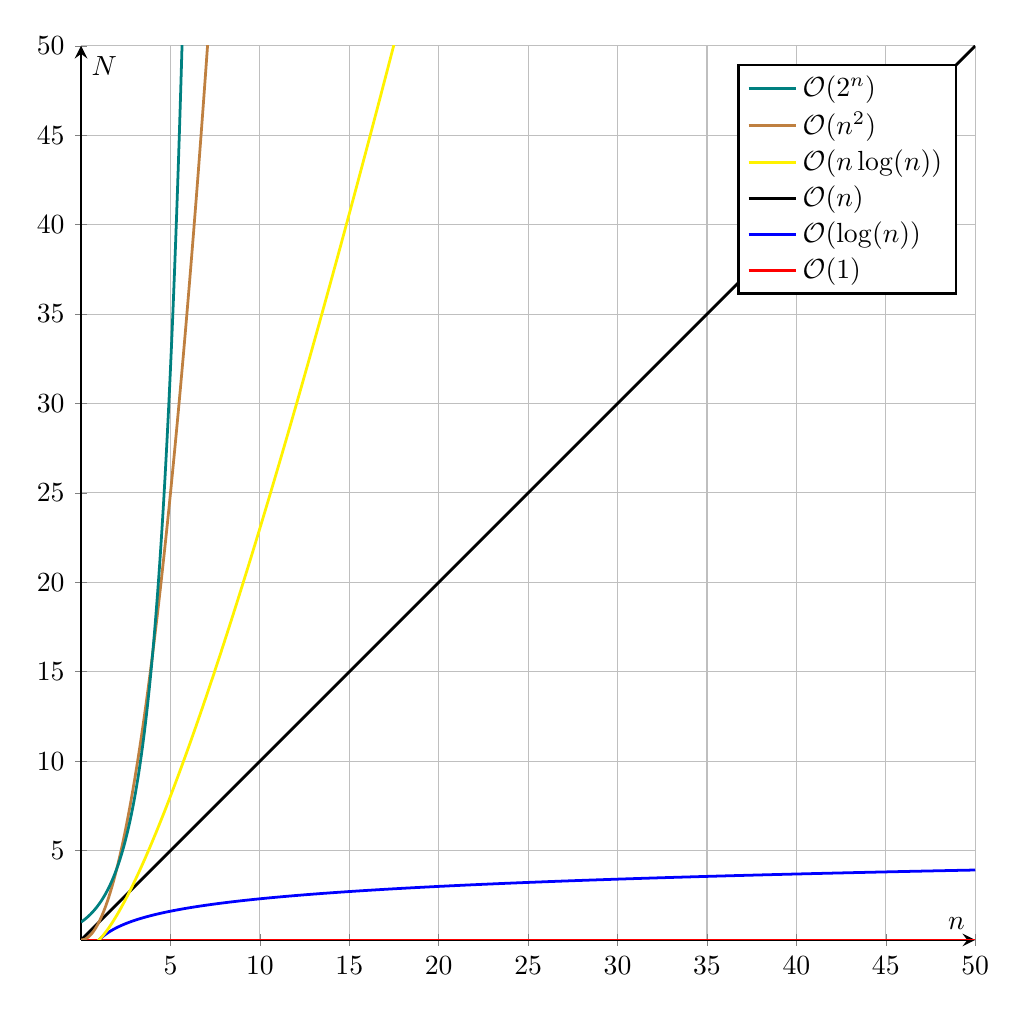
\begin{tikzpicture}[scale=1]
        \begin{axis}[
                width=15cm,
                unit vector ratio*=1 1,
                axis lines = middle,
                grid=major,
                ymin=0,
                ymax=50,
                xmin=0,
                xmax=50,
                xlabel = $n$,
                ylabel = $N$,
                xtick distance={5},
                ytick distance={5},
                disabledatascaling,
                cycle list name=color list,
                samples=250,
                solid,
                smooth,
                line width=1.0pt,
                no markers,
                legend cell align={left},
                reverse legend,
            ]

            \addplot +[domain=0:50]{0};         \addlegendentry{$\mathcal{O}(1)$};
            \addplot +[domain=0:50]{ln(x)};     \addlegendentry{$\mathcal{O}(\log(n))$};
                \addplot +[domain=0:50]{x};         \addlegendentry{$\mathcal{O}(n)$};
                \addplot +[domain=0:50]{x * ln(x)}; \addlegendentry{$\mathcal{O}(n \log(n))$};
            \addplot +[domain=0:50]{x^2};       \addlegendentry{$\mathcal{O}(n^2)$};
            \addplot +[domain=0:10]{2^x};        \addlegendentry{$\mathcal{O}(2^n)$};
        \end{axis}
    \end{tikzpicture}
\end{example}

\begin{example}[Komplexität]{Matrixmultiplikation}
    Problemgröße: $n$, ges.: $f(n)$ Anzahl der Rechen-Operationen in Abhängigkeit von der Matrix-Größe\\
    Notwendige Rechenzeit ist dann z.B.:
    \[T(n)=a\cdot f(n) + t_b\]
    mit $a$: Rechenzeit für eine Rechen- (Gleitkomma-) Operation,\\
    $b$: Rechenzeit für die Initialisierung und Beendigung des Algorithmus\\
    Formale Matrixmultiplikation:
    \[c_{i, j} = \sum\limits_{k=1}^{n}a_{i, k}\cdot b_{k, j}\]
    Bestimmung von $f(n)$: für jedes Element von $c$ sind $n$ Multiplikationen und $n-1$ Additionen durchzuführen.
    Also ergibt sich bei $n^2$ Elementen von $c$:
    \[f(n)=2\cdot n^3 - n^2\]

    TODO: Wording, Anschaulichkeit
\end{example}

\begin{bonus}{Master-Theorem}
    TODO
\end{bonus}

\begin{example}[Komplexität]{Strassen-Winograd}
    Effiziente Matrixmultiplikation:
    \begin{itemize}
        \item Matrizen werden in je vier Teilmatrizen der Größe $\frac{n}{2} \times \frac{n}{2}$ zerlegt:
              \begin{align*}
                  \begin{pmatrix}
                      A_{11} & A_{12} \\
                      A_{21} & A_{22}
                  \end{pmatrix}
                  \cdot
                  \begin{pmatrix}
                      B_{11} & B_{12} \\
                      B_{21} & B_{22}
                  \end{pmatrix}
                  =
                  \begin{pmatrix}
                      C_{11} & C_{12} \\
                      C_{21} & C_{22}
                  \end{pmatrix}
              \end{align*}
        \item Zusätzlich werden sieben neue Matrizen definiert:
              \begin{itemize}
                  \item $M_1 = (A_{12} - A_{22})\cdot(B_{21} + B_{22})$,
                  \item $M_2 = (A_{11} + A_{22})\cdot(B_{11} + B_{22})$,
                  \item $M_3 = (A_{11} - A_{21})\cdot(B_{11} + B_{12})$,
                  \item $M_4 = (A_{11} + A_{12})\cdot B_{22}$,
                  \item $M_5 = A_{11}\cdot(B_{21} - B_{22})$,
                  \item $M_6 = A_{22}\cdot(B_{21} - B_{11})$,
                  \item $M_7 = (A_{21} - A_{22})\cdot B_{11}$
              \end{itemize}
        \item Die vier Teilmatrizen der Ergebnismatrix ergeben sich damit wie folgt:
              \begin{itemize}
                  \item $C_{11} = M_1 + M_2 - M_4 + M_6$
                  \item $C_{12} = M_4 + M_5$
                  \item $C_{21} = M_6 + M_7$
                  \item $C_{22} = M_2 - M_3 + M_5 - M_7$
              \end{itemize}
    \end{itemize}
    Komplexität: $O(n^{\log_2 7})\approx O(n^2.807)$
\end{example}

\begin{defi}{Landau-Notation}
    Edmund Landau hat mit dem $O$-Symbol eine Notation geliefert,
    die den bestimmenden Term einer Funktion bezeichnet. \\
    $O(g(n))$ bezeichnet eine Klasse von Funktionen, wobei
    \[f(n) \in O(g(n))\]
    bedeutet, dass $f(n)$ höchstens so schnell wächst wie $g(n)$,
    das heißt, es gibt zwei positive Konstanten $c$ und $n_0$,
    für die gilt:
    \[|f(n)| \leq c \cdot |g(n)| \forall n \geq n_0\]
    (Definition hier nur für Funktionen über natürliche Zahlen)
\end{defi}

\begin{example}{Komplexitätsklassen}
    \begin{tabularx}{\textwidth}{|l|X|}
        \hline
        $O(1)$        & das Programm wird nur einmal linear durchlaufen, ohne von der Problemgröße abzuhängen (d.h. ohne Schleifen über $n$) $\to$ konstante Rechenzeit \\
        \hline
        $O(\log n)$   & z.B.\ bei Zerlegung von Problemen in Teilprobleme und Bearbeitung eines Teilproblems (binäre Suche)                                             \\
        \hline
        $O(n)$        & Algorithmen mit Schleifen $i = n_0 \ldots n$ (sequentielle Suche)                                                                               \\
        \hline
        $O(n \log n)$ & z.B.\ bei Zerlegung des Problems in Teilprobleme mit Bearbeitung aller Teilprobleme (Quicksort)                                                 \\
        \hline
        $O(n^2)$      & z.B.\ verschachtelte Schleifen (Paarweiser Vergleich)                                                                                           \\
        \hline
        $O(n^3)$      & z.B.\ dreifach verschachtelten Schleifen (Matrixmultiplikation)                                                                                 \\
        \hline
        $O(2n)$       & z.B.\ Suche in allen Kombinationen, Paaren oder Teilmengen                                                                                      \\
        \hline
    \end{tabularx}
\end{example}




\section{Parallelverarbeitung}\label{sec:parallelverarbeitung}

\subsection{Parallele Bearbeitung einer Aufgabe}

\begin{defi}{Parallelverarbeitung}
    % TODO: https://de.wikipedia.org/wiki/Nebenl%C3%A4ufigkeit (Quelle)
    Die \emph{Parallelverarbeitung} (engl. \enquote{concurrency}), zielt darauf ab, mehrere Aufgaben, Berechnungen, Anweisungen oder Befehle gleichzeitig ausführen zu können.
    Es kann sich dabei um völlig unabhängige Anweisungen handeln, bis hin zur gemeinsamen Bearbeitung einer Aufgabe.
    
    Ziel ist eine \emph{Leistungssteigerung}.
    
    Voraussetzungen sind, dass
    \begin{itemize}
        \item eine Aufteilungsmöglichkeit existiert und erkannt wird,
        \item mehrere Bearbeiter zur Verfügung stehen und
        \item diese gleichzeitig und dabei möglichst unabhängig agieren können.
    \end{itemize}
\end{defi}

\begin{defi}{Domain Decomposition}
    \emph{Domain Decomposition} bzw. \emph{Gebietszerlegung} beschreibt die statische oder dynamische Aufteilung eines Datengebiets in Bereiche gleicher Prozessorarbeit.
    Alle Gebiete werden mit demselben Programmteil parallel verarbeitet.
    
    Domain Decomposition ist insbesondere geeignet für \emph{homogene Plattformen}.
    
    Im High-Performance-Computing (HPC) wird diese Art der Parallelisierung häufigsten verwendet.
\end{defi}

\begin{defi}[Domain Decomposition]{Statische Aufteilung}
    % TODO: https://de.wikipedia.org/wiki/Lastverteilung_(Informatik) (Quelle)
    \emph{Statische Aufteilung} der Domain Decomposition berücksichtigt den Zustand verschiedener Maschinen nicht.
    Sie soll z. B. die Kommunikation zwischen Prozessoren minimieren, oder bestimmte Hardware-Eigenschaften des Verbindungsnetzwerkes ausnutzen.
    
    Der Vorteil statischer Aufteilung ist, dass sie leicht zu implementieren und bei relativ regelmäßigen Aufgaben äußerst effizient ist.
\end{defi}

\begin{example}[Domain Decomposition]{Statische Aufteilung}
    TODO: Grafik
\end{example}

\begin{defi}[Domain Decomposition]{Dynamische Aufteilung}
    % TODO: https://de.wikipedia.org/wiki/Lastverteilung_(Informatik) (Quelle)
    \emph{Dynamische Aufteilung} der Domain Decomposition soll ein Gebiet in Bereiche gleicher Prozessorarbeit aufteilen.
    
    Im Gegensatz zur statischen Aufteilung wird bei der dynamische Variante die aktuelle Last jeder der Recheneinheiten im System berücksichtigt.
    Bei diesem Ansatz können Aufgaben dynamisch von einem überlasteten Knoten zu einem unterlasteten Knoten verschoben werden, um eine schnellere Verarbeitung zu erhalten.
    
    Obwohl diese Algorithmen viel komplizierter zu entwerfen sind, können sie hervorragende Ergebnisse liefern, insbesondere wenn die Ausführungszeit von einer Aufgabe zur anderen stark variiert.
    
\end{defi}

\begin{example}[Domain Decomposition]{Dynamische Aufteilung}
    TODO: Grafik
\end{example}

\begin{defi}{Functional Decomposition}
    \emph{Functional Decomposition} bzw. \emph{Funktionsaufteilung} beschreibt die Zerlegung eines Problems in unterschiedliche Programmteile, Unterprogramme oder Module, die dann auf Prozessoren verteilt und parallel bearbeitet werden.
    
    Dabei können die Programmteile auf jeweils unterschiedlichen, eventuell spezialisierten, Rechnerarchitekturen ausgeführt werden.
\end{defi}

\begin{jsc}[Functional Decomposition]{Modulare Supercomputing Architektur}
    % TODO: https://www.fz-juelich.de/de/ias/jsc/ueber-uns/struktur/forschungsgruppen/jsc-rg-proto/modulare-supercomputing-architektur (Quelle)
    Die \emph{Modular Supercomputing Architecture} (\emph{MSA}) ist ein Systemdesign zur Integration heterogener Ressourcen und zur Erfüllung der Anforderungen eines breiten Spektrums von Anwendungsbereichen, die von rechenintensiven, hochskalierenden Simulationscodes bis hin zu datenintensiven Workflows der künstlichen Intelligenz reichen.
    
    \vspace{1em}
    
    \centering
    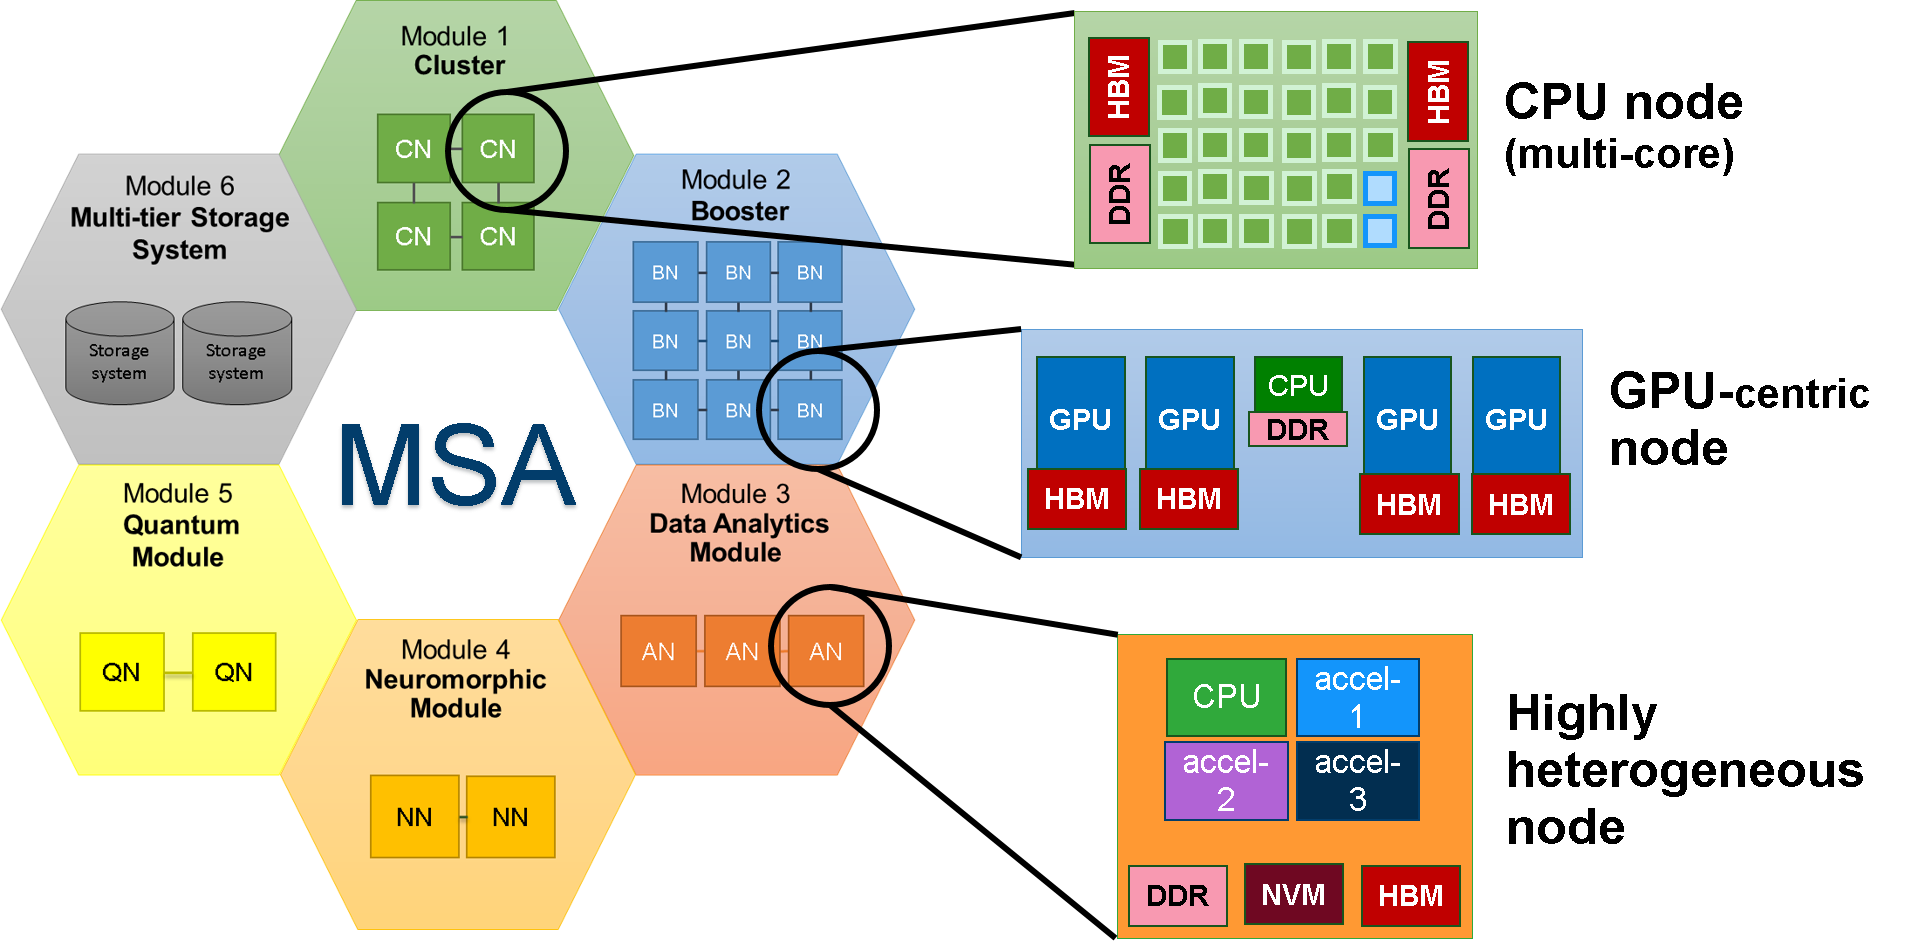
\includegraphics[width=0.9\linewidth]{images/modular_supercomputing_architecture.png}
\end{jsc}

\subsection{Speedup, Effizienz, Skalierbarkeit}

\begin{defi}{Speedup}
    % TODO: https://de.wikipedia.org/wiki/Speedup
    \emph{Speedup} beschreibt mathematisch den Zusammenhang zwischen der seriellen und der parallelen Ausführungszeit eines Programmteils.
    
    Der \emph{reale Speedup} $S$ einer parallelen Ausführung, der zur realen Messung herangezogen wird, kann wie folgt definiert werden:
    \[
        S = \frac{t_S}{t_p}
    \]
    Dabei sind $t_S$ und $t_p$ die serielle bzw. die parallele Ausführungszeit bei $p$ parallelen Bearbeitungseinheiten (Prozessoren).
\end{defi}

\begin{defi}{Amdahl's Law}
    % TODO: https://de.wikipedia.org/wiki/Speedup (Quelle)
    % TODO: https://de.wikipedia.org/wiki/Amdahlsches_Gesetz (Quelle)
    Das \emph{Amdahlsche Gesetz} (engl. \emph{Amdahl's Law}) ist ein Modell über die Beschleunigung von Programmen durch parallele Ausführung.
    Nach Amdahl wird der Geschwindigkeitszuwachs vor allem durch den sequentiellen Anteil des Problems beschränkt, da sich dessen Ausführungszeit durch Parallelisierung nicht verringern lässt.
    
    Der \emph{theoretische Speedup} $\eta_S$ nach Amdahl kann wie folgt definiert werden:
    \[
        \eta_S = \frac{t_S}{t_S \cdot f + t_S \cdot \frac{1-f}{p} } = \frac{t_S}{t_S \left((1 - f) + \frac{f}{n_P}\right)}
    \]
    Dabei sind $t_S$ und $t_p$ die serielle bzw. die parallele Ausführungszeit bei $p$ parallelen Bearbeitungseinheiten (Prozessoren);
    $f$ ist der Anteil der Laufzeit bzw. des Programms, der nicht parallel ablaufen kann und $n_P$ die Anzahl der Anzahl der Prozessoren, die zur Berechnung eingesetzt werden können.
    
    Es gelten weiterhin folgende Grenzwerte:
    \[
        \lim_{p \to \infty} \eta_S = \frac{1}{f} \quad \text{und} \quad \lim_{f \to 0 } \eta_S = n_P
    \]
\end{defi}

\begin{bonus}{Durchsatz}
    \emph{Durchsatz} ist ein Maß für die Bewertung der Verarbeitung einer gesamten Arbeitslast
    (mit welchem Flugzeug kann eine Fluggesellschaft mehr Personen befördern ?).
\end{bonus}

\begin{defi}{Effizienz}
    \emph{Effizienz} definiert das Verhältnis von Speedup und eingesetzter Prozessoranzahl.
    Sie drückt aus, welcher Anteil der Prozessorleistung nutzbar ist.
    
    Sie kann definiert werden als:
    \[
        E = \frac{S}{n_P} = \frac{t_S}{n_P\cdot t_P} \in (0; 1)
    \]
    \begin{align*}
        E(p) = \frac{S(p)}{p} =
        \frac{T(\text{sequentiell})}{p\cdot T(\text{parallel})},
        0<E(p)\leq 1
    \end{align*}
\end{defi}

\begin{example}[Speedup]{Skalarprodukt}
    Paralleler Algorithmus:
    \begin{enumerate}
        \item Aufteilen in $p$ Teilvektoren der Länge $\frac{n}{p}$
        \item jeder Prozessor berechnet das Skalarprodukt des Teilvektors $T_* (p) = \left(2 \cdot \frac{n}{p} - 1\right) \cdot t_\text{flop}$
        \item die Ergebnisse werden zu Prozessor 1 übertragen $T_t (p) = (p - 1) \cdot (t_\text{startup} + t_\text{word})$
        \item und Addition der Teilergebnisse (reduzieren) $T_+ (p) = (p - 1) \cdot t_\text{flop}$
    \end{enumerate}
    für $p=2^d$:
    \begin{align*}
        S(p) = \frac{T(\text{seq})}{T(p)} = \ldots =
        \frac{p}{\frac{p(\frac{2n}{p} + d-1)}{2n-1} + \frac{p\cdot d\cdot (t_\text{startup} + t_\text{word})}{(2n - 1)t_\text{flop}}}
    \end{align*}
    bei $n\gg p$:
    \begin{align*}
        \approx\frac{p}{
        \underbrace{1 + p\cdot \log_2 p}_{\text{Algorithmus}} \cdot
        \underbrace{\frac{1}{2n}}_{\text{Problemgröße}} \cdot
        \underbrace{\frac{t_\text{startup}}{t_\text{flop}}}_{\text{Hardware}}}
    \end{align*}
    
    TODO: Darstellung
\end{example}

\begin{example}[Effizienz]{Skalarprodukt}
    \[
        E(p) \approx \frac{1}{1 + n_P \cdot \log_2 n_P \cdot \frac{1}{2n} \cdot \frac{t_\text{startup}}{t_\text{flop}}}
    \]
    Die Effizienz
    \begin{itemize}
        \item \emph{steigt} mit wachsender Problemgröße $n$ (bei $n_P$ fest) und
        \item \emph{sinkt} bei größerer Prozessoranzahl $n_p$ (mit $n$ fest).
    \end{itemize}
    
    TODO: Darstellung\\
    TODO: Wie muss die Problemgröße $n$ wachsen bei festem $n_P$ und konstanter Effizienz?
\end{example}

\begin{defi}{Skalierbarkeit}
    Eine Rechnerarchitektur bzw. ein Programm ist \emph{skalierbar}, wenn die Effizienz der Programmbearbeitung bei wachsender Prozessorzahl gleich bleibt.
    Dies kann im Allgemeinen nur durch gleichzeitige Vergrößerung der Problemgröße erfolgen.
    
    Ein Programm bzw. ein Algorithmus ist \emph{perfekt skalierbar}, wenn $n \in \mathcal{O}(n_P)$ ist, also linear in $n_P$.
    
    TODO: Was soll das heißen?
\end{defi}

\begin{defi}{Paralleler Overhead}
    
    Der Speedup kann sich reduzieren durch zusätzlichen \emph{parallelen Overhead}.
    
    \[
        V(n_P) = n_P \cdot t_P - t_S
    \]
    
    Der \emph{durchschnittliche parallele Overhead} ist definiert als:
    \[
        \overline{V}(n_P) = \frac{V(n_P)}{n_P}
    \]
    
    Er wird verursacht durch:
    \begin{itemize}
        \item Kosten für das Starten eines Vorgangs (\enquote{startup}),
        \item Kosten für das Verteilen bzw. Verwalten gemeinsamer Daten, oder
        \item Kosten für Synchronisation.
    \end{itemize}
    
    Daher gilt abzuwägen zwischen:
    \begin{itemize}
        \item Verkleinern der Kommunikation durch größere Arbeitspakete (\emph{grobkörnige Granualität})
        \item Kleine Arbeitspaketen, damit viele Prozessoren arbeiten (\emph{feinkörnige Granualität})
    \end{itemize}
    
    TODO: Sinnvolle Definition finden
\end{defi}

\subsection{Aufgaben}

\begin{aufgabe}{Speedup}
    Ein sequentielles Programm lasse sich zu $80\%$ parallelisieren. 
    Welcher Speedup kann mit 20 Prozessoren erzielt werden?
    \tcblower
    Der Speedup ist definiert durch: 
    \begin{align*}
        \eta_S = \frac{t_S}{t_S \cdot f + t_S \cdot \frac{1-f}{p}}
    \end{align*}
    mit $t_S=1$, $f=1-0.8=0.2$, $p=20$ ist der Speedup eines Programmes dann:
    \begin{align*}
        \eta_S = \frac{1}{1 \cdot 0.2 + 1 \cdot \frac{0.8}{20}} = \frac{25}{6} \approx 4.1667
    \end{align*}
\end{aufgabe}

\begin{aufgabe}{Skalierbarkeit}
    Wann ist eine Rechnerarchitektur bzw. ein Programm skalierbar?
    \tcblower
    Wenn die Effizienz der Programmbearbeitung bei wachsender Prozessorzahl gleich bleibt.
\end{aufgabe}

\begin{aufgabe}{Pipelining}
    Wie berechnet sich der Speedup $\eta_S$ bei Pipeline-Nutzung mit n Aufträgen und k Stufen?
    \tcblower
    Der Speedup berechnet sich durch: 
    \begin{align*}
        \eta_S = \frac{n\cdot k}{n+k-1}
    \end{align*}
\end{aufgabe}

\section{Einzelprozessorsysteme}\label{sec:einzelprozessorsysteme}

\begin{defi}{Überlappte Verarbeitung}
    Erstes Ziel war die überlappte Verarbeitung von langsamen und schnellen Hardware-Komponenten. 
    (Verstecken der langsamen Funktionseinheiten)
\end{defi}

\begin{defi}{Überlappter I/O}
    Während des langsamen I/O kann nun gleichzeitig die \enquote{wertvolle} Ressource CPU genutzt werden.
\end{defi}

\subsection{Cache}\label{subsec:cache}

\begin{defi}{Cache}
    \ldots ist ein schneller Speicher mit verhältnismäßig kleiner Speicherkapazität, 
    der zwischen der Zentraleinheit (CPU) und dem Arbeitsspeicher positioniert ist.
\end{defi}

\begin{defi}{Direct Mapped Cache}
    Feste Abbildung der Hauptspeicher-Adressen auf die Cache-Adressen
    \begin{itemize}[$\to$]
        \item Kein assoziativer Speicher nötig
        \item Keine Verdrängungsstrategien nötig
    \end{itemize}
\end{defi}

\begin{defi}{N-way Set Associative Cache}
    N-fache Mengenassoziativität: $N$ Einträge pro Cache-Index\\
    $\to$ $N$ Caches mit direkter Abbildung, die parallel operieren
    ($N$ liegt meist zwischen 2 und 4)\\
    Beispiel: zweifach mengenassoziativer Cache
    \begin{itemize}
        \item Der Cache-Index bestimmt eine \enquote{Menge} von Blöcken im Cache
        \item Die beiden Tags werden parallel verglichen.
        \item Die Daten werden aufgrund des Tagvergleichs selektiert.
    \end{itemize}
\end{defi}

\begin{defi}{Fully Associative Cache}
    
\end{defi}

\begin{defi}{Ersetzungsstrategie}
    \begin{itemize}
        \item Trivial für Direct Mapped Cache
        \item Bei Set Associative oder Fully Associative:
        \begin{itemize}
            \item Random
            \item LRU (Least Recently Used) bzw. FIFO
        \end{itemize}
    \end{itemize}
    Zurückschreiben von Daten:
    \begin{itemize}
        \item \underline{Write through:} Die Information wird sowohl in den Cache als auch ins
        Memory zurückgeschrieben.
        \item \underline{Write back:} Die Information wird nur in den Cache geschrieben. Die
        veränderte Zeile wird erst dann ins Memory geschrieben, wenn die
        Cache-Zeile mit Daten aus anderen Hauptspeicheradressen
        überschrieben werden soll.
        \begin{itemize}
            \item \underline{Vorteil:} Mehrfaches Ändern eines Wertes wird nur im Cache durchgeführt.
            \item \underline{Nachteil:} Ein Read-Miss kann zu einem Schreiben ins Memory führen.
        \end{itemize}
    \end{itemize}
\end{defi}

\begin{bonus}[Cache]{IBM Power 4}
    
\end{bonus}

\begin{bonus}[Cache]{Intel Itanium}
    
\end{bonus}

\begin{defi}{Cache Miss}
    Ist keine Kopie der Hauptspeicherzelle a im Cache abgelegt, so 
    \begin{itemize}
        \item greift die CPU auf den Arbeitsspeicher zu,
        \item lädt das Datum in den Cache und
        \item lädt das Datum gleichzeitig in die CPU.
    \end{itemize}
\end{defi}

\begin{defi}{Reduzierung der Cache Miss Rate}
    \begin{itemize}
        \item \underline{Cold start miss:} Tritt auf beim ersten Zugriff auf einen Block nach dem Start des Programms oder dem Task-Wechsel (auch bei unendlich großem Cache)
        \item \underline{Capacity miss:} Tritt auf, wenn der Cache nicht alle Blocks speichern kann, die bei der Ausführung durch die CPU benötigt werden (nur bei fully associative Cache)
        \item \underline{Conflict miss:} Tritt auf, wenn ein Block ersetzt werden muß, der anschließend wieder benötigt wird (bei N-way associative Cache)
        \item \underline{Coherence miss:} bei Mehrprozessorsystemen → wird später erklärt
    \end{itemize}
\end{defi}

\begin{defi}[Reduzierung der Cache Miss Rate]{Programmierstrategien}
    Verbessern der Speicherlokalität durch
    \begin{itemize}[\ldots]
        \item Datenstrukturierung
        \item Ändern der Indexierung
        \item Schleifenfusion
        \item Bildung von Teilblöcken
    \end{itemize}
\end{defi}

\begin{defi}{Table-Look-Aside Buffer}
    Bei Rechnern mit virtueller Speicherverwaltung arbeitet der Prozessor mit virtuellen Adressen, 
    die durch den TLB in reale Adressen umgesetzt werden.
\end{defi}

\subsection{Entwicklungslinien der Prozessoren}\label{subsec:entwicklungslinien-der-prozessoren}

\begin{defi}{Complex Instruction Set Computer (CISC)}
    Befehls-Code ist Index auf Zeiger-Array für Mikroprogramm,
    die Hardware führt die Sequenz der Mikrobefehle aus.
\end{defi}

\begin{defi}{Reduced Instruction Set Computer (RISC)}
    Der Compiler erzeugt direkt \enquote{Mikrobefehle}. 
    Es muss zwar mehr Code erzeugt werden, 
    aber die Hardware wird einfacher und damit auch schneller.
\end{defi}

\begin{defi}{Very Long Instruction Word (VLIW)}
\end{defi}

\begin{defi}{Explicitly Parallel Instruction Computing (EPIC)}
    Von HP und Intel wurde 1998/99 die Prozessorarchitektur EPIC entworfen 
    und mit dem Intel Itanium ein erster Prozessor realisiert. 
    Die Intel-Version der Architektur wird IA-64 (64 bit) genannt.

    EPIC ist die moderne Weiterentwicklung des Konzepts des VLIW.
    
    Hierbei versucht der Compiler, 
    möglichst viele voneinander unabhängige Instruktionen in einer Sequenz zusammenzustellen. 
    Er kann dabei durch Umstellen der Befehle die Reihenfolge innerhalb der Sequenz verändern. 
    Dies darf aber nicht zu anderen Ergebnissen führen!
    
    Eine solche Sequenz nennt Intel ein “bundle”.
\end{defi}

\section{Pipelining}

\begin{defi}{Pipelining}
    Durch Aufteilen einer Instruktion in Teile, 
    die in separaten Funktionseinheiten bearbeitet werden können, 
    ist eine überlappte (pseudo-parallele) Verarbeitung der Instruktionen möglich.
\end{defi}

\begin{defi}[Pipelining]{Funktionseinheiten}
    Eine 5-stufige Pipeline (z.B. MIPS-Prozessor) wird aus folgenden Funktionseinheiten gebildet:
    \begin{center}
        \begin{tabular}{ll}
            IF:  & Instruction Fetch  \\
            ID:  & Instruction Decode \\
            EX:  & Execution          \\
            MEM: & Memory Access      \\
            WB:  & Write Back         \\
        \end{tabular}
    \end{center}
\end{defi}

\begin{defi}[Pipelining]{Latenz}
    Wie groß ist die Laufzeit für eine einzelne Instruktion?
    \[T_\text{instr} = T_\text{IF} + T_\text{ID} + T_\text{EX} + T_\text{MEM} + T_{WB}\]
\end{defi}

\begin{defi}[Pipelining]{Durchsatz}
    Wie oft pro Zeiteinheit wird eine Instruktion fertig ?
    \[X = \frac{1}{\max(T_\text{IF}, T_\text{ID}, T_\text{EX}, T_\text{MEM}, T_{WB})}\]
\end{defi}

\begin{defi}{Superskalarität}
    
\end{defi}

\begin{defi}{Instruction Level Parallelism (ILP)}
    Ziel bei ILP ist es, 
    alle Funktionseinheiten aller Pipelines ohne Unterbrechungen (bubbles) ständig arbeiten zu lassen.
\end{defi}

\begin{defi}{Hazards}
    \begin{itemize}
        \item \underline{Structural hazards:}
              Die HW kann nicht eine bestimmte Aufeinanderfolge von Instruktionen ausführen.
        \item \underline{Data hazards:}
              Instruktionen hängen vom Ergebnis vorheriger Schritte ab, 
              die noch nicht die Pipeline verlassen haben.
        \item \underline{Control hazards:}
              Zwischen dem \enquote{fetch} von Instruktionen und dem Ändern des Kontrollflusses (branch) entstehen Verzögerungen.
    \end{itemize}
\end{defi}

\begin{defi}{Schleifenparallelisierung}
    Ziel ist es, 
    den Schleifenkörper ohne stottern durch die vorhandenen Funktionsinheiten zu schicken.
    Dazu sind Abhängigkeiten zwischen den Anweisungen zu finden und, 
    wenn möglich, zu beseitigen.
\end{defi}

\begin{defi}{Abhängigkeitsgraph}
    
\end{defi}

\begin{defi}{Predication}
    Mit der Predication-Methode können bestimmte Control Hazards (branches) aufgelöst werden, 
    z. B. 'If-then-else'-Konstrukte
\end{defi}

\begin{defi}{Data Speculation}
    Durch Umstellen der Befehlsreihenfolge (z. B. Laden von Daten) kann Parallelität erhöht werden.
\end{defi}

\begin{defi}{Control Speculation}
    Durch Umstellen der Befehlsreihenfolge (z. B. Ausführung von Operationen) kann Parallelität erhöht werden.
\end{defi}

\begin{defi}{Attached-Processor-Systeme}
    Eine zusätzliche Einheit, 
    die in einer Multiprozessor-Umgebung an die primäre CPU angeschlossen ist. 
    Sie arbeitet als Erweiterung der primären CPU und 
    nutzt die Systemsoftware und Peripheriegeräte gemeinsam.
\end{defi}
\section{Mehrprozessorsysteme}

\begin{defi}{Flynn'sche Klassifikation}
    Von Flynn wurde 1972 eine sehr grobe aber heute noch häufig genutzte Unterscheidung von Parallelrechnern eingeführt.
    Sie orientiert sich an der Anzahl der gleichzeitig vorhandenen Instruktions- und Datenströme.
    
    Parallelrechner:
    
    \begin{center}
        \begin{tabular}{ll}
            SISD & Single Instruction Single Data (Von Neumann-Rechner $\to$ kein paralleles System) \\
            SIMD & Single Instruction Multiple Data                                                  \\
            MISD & Multiple Instruction Single Data $\to$ \textbf{irrelevant!}                       \\
            MIMD & Multiple Instruction Multiple Data 
        \end{tabular}
    \end{center}
\end{defi}

\begin{bonus}[Flynn'sche Klassifikation]{Erweiterungen}
    \begin{itemize}
        \item \emph{SIMD} Single Instruction Multiple Data
              \begin{itemize}
                  \item Vektor-Prozessoren (auch Mischformen mit MIMD vorhanden!)
                  \item Array-Prozessoren
              \end{itemize}
        \item \emph{MIMD} Multiple Instruction Multiple Data
              \begin{itemize}
                  \item Speichergekoppelte Multiprozessoren
                        \begin{itemize}
                            \item Unified Memory Architecture (UMA)
                            \item Non-Uniform Memory Access (NUMA)
                        \end{itemize}
                  \item Nachrichtengekoppelte Multiprozessoren
                        \begin{itemize}
                            \item Massively Parallel Processing (MPP)
                            \item Cluster Of Workstations (COW)
                        \end{itemize}
              \end{itemize}
    \end{itemize}
\end{bonus}

\subsection{Speichergekoppelte Systeme}

\begin{defi}{Speichergekoppelte Systeme}
    Bei speichergekoppelten Multiprozessoren arbeiten alle Prozessoren in einem einheitlichen Adressraum.
    
    Je nach physiklischer Speicherorganisation unterscheidet man:
    \begin{itemize}
        \item Symmetrische Multiprozessoren (SMP, symmetric multiprocessor),
              bei denen gleichartige Prozessoren über ein Verbindungsnetzwerk mit einem gemeinsamen Speicher verbunden sind
        \item Distributed-Shared-Memory Systeme,
              bei denen zwar ein einheitlicher Adressraum existiert, 
              aber die Speicher physikalisch auf einzelnen Verarbeitungsknoten verteilt sind
    \end{itemize}
    
    \emph{Bemerkungen:}
    \begin{itemize}
        \item Speichergekoppelte Multiprozessoren gelten als einfacher programmierbar gegenüber nachrichtengekoppelten Multiprozessoren
        \item Nutzbare Parallelität reicht von der Programmebene bis zur Blockebene
        \item Autoparallelisierende Compiler nutzen insbesondere die Parallelisierung der Schleifenebene (einzelne Iterationen nebenläufig abarbeitbar)
    \end{itemize}
\end{defi}

\begin{defi}{Uniform Memory Access}
    Kapitel 5 Seite 8
\end{defi}

\begin{defi}{Non-Uniform Memory Access}
    Kapitel 5 Seite 9
\end{defi}

\begin{defi}{Nachrichtengekoppelte Systeme}
    Kapitel 5 Seite 10
\end{defi}

\subsection{Verbindungsnetzwerke}

\begin{defi}{Verbindungsnetzwerk}
    Ein Verbindungsnetzwerk ermöglicht den Datenaustausch (und die Verteilung des Programms) zwischen den Prozessoren.
    
    Um einen hohen Datentransfer zu erhalten, 
    wird eine große Anzahl von Drähten benötigt!
    
    Ein VN gleicht einer Straße:
    \begin{itemize}
        \item Link = Straße
        \item Switch = Kreuzung
        \item Distance/Hops = Anzahl der zurückgelegten Straßenblöcke
        \item Routing algorithm = Reiseplan
    \end{itemize}
    
\end{defi}

\begin{defi}[Verbindungsnetzwerk]{Latenz}
    Zeit für den Transfer zwischen den Knoten
\end{defi}

\begin{defi}[Verbindungsnetzwerk]{Bandbreite}
    \[\frac{\text{transferierte Daten}}{\text{Zeit}}\]
    Bandbeite eines Link: $\text{bw} = w \cdot \frac{1}{t}\frac{\text{bit}}{\text{sec}}$
    mit $w$: Anzahl der Drähte
\end{defi}

\begin{defi}[Verbindungsnetzwerk]{Durchmesser}
    Der \emph{Durchmesser} ist die maximale Distanz zwischen zwei beliebigen Prozessoren.
\end{defi}

\begin{defi}[Verbindungsnetzwerk]{Topologie}
    Die Topologie beschreibet, 
    wie die Nachbarknoten angeordnet und erreichbar sind?
\end{defi}

\subsubsection{Statische Verbindungsnetzwerke}

\begin{defi}{Lineare Anordnung}
    \begin{center}
        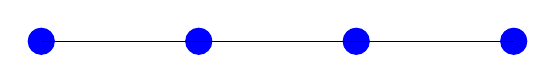
\begin{tikzpicture}
            \node[circle, draw=blue, fill=blue] (d0) at (0, 0) {};
            \node[circle, draw=blue, fill=blue] (d1) at (2, 0) {};
            \node[circle, draw=blue, fill=blue] (d2) at (4, 0) {};
            \node[circle, draw=blue, fill=blue] (d3) at (6, 0) {};
            \draw (d0.center) to[out=0, in=180] (d1.center);
            \draw (d1.center) to[out=0, in=180] (d2.center);
            \draw (d2.center) to[out=0, in=180] (d3.center);
        \end{tikzpicture}
        \\
        Diameter = $N-1$
    \end{center}
\end{defi}

\begin{defi}{Torus oder Ring}
    \begin{center}
        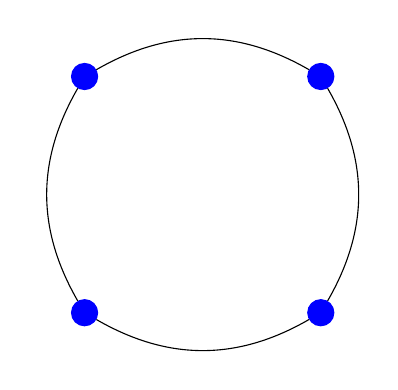
\begin{tikzpicture}
            \node[circle, draw=blue, fill=blue] (d0) at (3.5, 0.5) {};
            \node[circle, draw=blue, fill=blue] (d1) at (3.5, 3.5) {};
            \node[circle, draw=blue, fill=blue] (d2) at (0.5, 3.5) {};
            \node[circle, draw=blue, fill=blue] (d3) at (0.5, 0.5) {};
            \draw (d0) to[bend right] node[left]{}(d1);
            \draw (d1) to[bend right] node[left]{}(d2);
            \draw (d2) to[bend right] node[left]{}(d3);
            \draw (d3) to[bend right] node[left]{}(d0);
        \end{tikzpicture}
        \\
        Diameter = $\frac{N}{2}$
    \end{center}
\end{defi}

\begin{defi}{Torus}
    2D-Torus:
    \begin{center}
        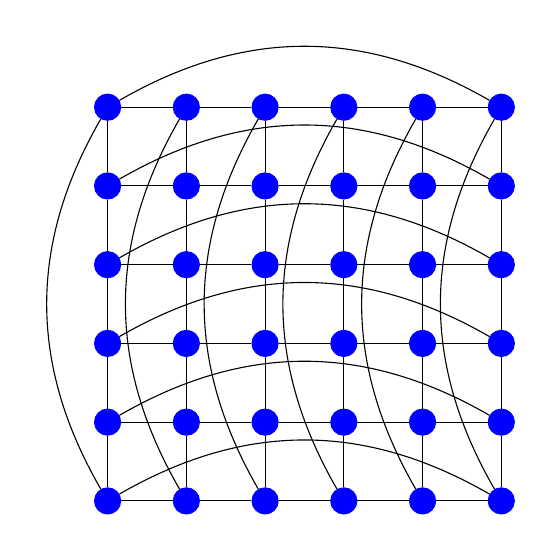
\begin{tikzpicture}[circlestyle/.style={circle, draw=blue, fill=blue}]
            \foreach \x in {0, ..., 5}
            \foreach \y in {0, ..., 5}
            \node[circlestyle] (\x\y) at (\x, \y) {};
            
            \foreach \x in {0,...,5}
            \foreach \y [count=\yi] in {0,...,4}
            \draw (\x\y)--(\x\yi) (\y\x)--(\yi\x); 
            
            \draw (00) to[bend left] node[left]{}(05);
            \draw (10) to[bend left] node[left]{}(15);
            \draw (20) to[bend left] node[left]{}(25);
            \draw (30) to[bend left] node[left]{}(35);
            \draw (40) to[bend left] node[left]{}(45);
            \draw (50) to[bend left] node[left]{}(55);
            
            \draw (00) to[bend left] node[left]{}(50);
            \draw (01) to[bend left] node[left]{}(51);
            \draw (02) to[bend left] node[left]{}(52);
            \draw (03) to[bend left] node[left]{}(53);
            \draw (04) to[bend left] node[left]{}(54);
            \draw (05) to[bend left] node[left]{}(55);
        \end{tikzpicture}
    \end{center}
\end{defi}

\begin{defi}{Gitter}
    2D-Gitter:\\
    Diameter = $2\cdot\left(\sqrt{N} - 1\right)$
    \begin{center}
        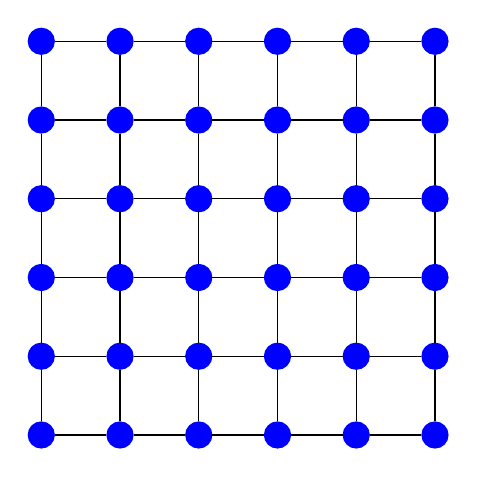
\begin{tikzpicture}[circlestyle/.style={circle, draw=blue, fill=blue}]
            \foreach \x in {0, ..., 5}
            \foreach \y in {0, ..., 5}
            \node[circlestyle] (\x\y) at (\x, \y) {};
            
            \foreach \x in {0,...,5}
            \foreach \y [count=\yi] in {0,...,4}
            \draw (\x\y)--(\x\yi) (\y\x)--(\yi\x); 
        \end{tikzpicture}
    \end{center}
\end{defi}

\begin{defi}{Hypercube}
    \begin{itemize}
        \item Anzahl der Knoten: $N = 2d$
        \item Diameter: $d = \log_2 N$
        \item Greycode Adressierung: Jeder Knoten verbunden mit $d$ anderen Knoten unterscheidet sich durch \emph{ein Bit} in der Adresse
        \item Beispiele: Intel iPSC und NCUBE
        \item Visualisierungen: \\
              \begin{tabular}{|c|c|c|c|}
                  \hline
                  
\begin{tikzpicture}[circlestyle/.style={circle, draw=blue, fill=blue}]
                      \node[circlestyle] (A) at (0,0) {};
                  \end{tikzpicture} & 
                  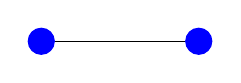
\begin{tikzpicture}[circlestyle/.style={circle, draw=blue, fill=blue}]
                      \node[circlestyle] (A) at (0,0) {};
                      \node[circlestyle] (B) at (2,0) {};
                      \draw (A) to[] node[left]{}(B);
                  \end{tikzpicture} & 
                  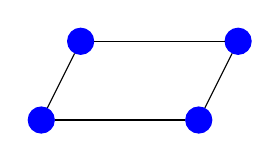
\begin{tikzpicture}[circlestyle/.style={circle, draw=blue, fill=blue}]
                      \node[circlestyle] (A) at (0,0) {};
                      \node[circlestyle] (B) at (2,0) {};
                      \draw (A) to[] node[left]{}(B);
                      
                      \node[circlestyle] (C) at (0.5, 1) {};
                      \node[circlestyle] (D) at (2.5, 1) {};
                      \draw (C) to[] node[left]{}(D);
                      
                      \draw (A) to[] node[left]{}(C);
                      \draw (B) to[] node[left]{}(D);
                  \end{tikzpicture} & 
                  TODO !                                    \\
                  0d                         & 1d & 2d & 4d \\
                  \hline
              \end{tabular}
    \end{itemize}
\end{defi}

\begin{defi}{Baum}
    Diameter = $\log_2 N$
    \begin{itemize}
        \item Planares Layout:
              TODO: tikzpicture
        \item Fetter Baum: (mehr Verbindungen erhöhen das Datenvolumen)
    \end{itemize}
\end{defi}

\begin{bonus}{Übersicht statischer Verbindungsnetzwerke}
    \begin{tabularx}{\textwidth}{|l|X|X|X|}
        \hline
        Topologie          & Anzahl der Verbindungskanäle pro Knoten & Maximale Entfernung (Diameter) & Gesamtanzahl der Verbindungskanäle \\
        \hline
        Ring               & 2                                       & $\frac{N}{2}$                  & $N-1$                              \\
        \hline
        Baum               & 3                                       & $2\cdot (\log_2 N - 1)$        & $N-1$                              \\
        \hline
        2D - Gitter        & 4                                       & $2\cdot \sqrt{N}$              & $2\cdot N$                         \\
        \hline
        3D - Gitter        & 6                                       & $3\cdot \sqrt[3]{N}$           & $3\cdot N$                         \\
        \hline
        Hexagon. Gitter    & 6                                       & $3\cdot \sqrt[3]{N}$           & $3\cdot N$                         \\ 
        \hline
        Hypercube          & $\log_2 N$                              & $\log_2 N$                     & $N \log_2 \frac{N}{2}$             \\
        \hline
        Vollst. Vernetzung & $N - 1$                                 & 1                              & $N \cdot \frac{N-1}{2}$            \\
        \hline
    \end{tabularx}
\end{bonus}

\subsubsection{Dynamische Verbindungsnetzwerke}

\begin{defi}{Bus}
    \begin{itemize}
        \item Durch die wahlweise Zuschaltung einzelner Verarbeitungsknoten zum Datentransfer an einen Bus ist das Bussystem eine typische dynamische Verbindungseinrichtung
        \item Der Bus bildet die Engstelle im busgekoppelten Multiprozessorsystem,
              so dass auch Doppelbusse oder allgemein Mehrfachbusse eingesetzt werden
        \item Bussysteme und auch Mehrbussysteme werden für Systeme mit höchstens 30 Prozessoren eingesetzt,
              um Zugiffskonflikte in Grenzen zu halten
    \end{itemize}
\end{defi}

\begin{defi}{Crossbar}
    \begin{itemize}
        \item $M \times M$ Matrix
        \item einfaches Weiterleiten an mehrere Ausgänge
        \item komplexe Steuerung
        \item Verdrahtungsaufwand
        \item Pufferung bei Blockierungen
        \item Diameter = 1, d. h. beliebige Verbindungen können unter Einsatz jeweils nur einer Schaltzelle realisiert werden
    \end{itemize}
\end{defi}

\begin{defi}{Zellenbasierte Systeme}
    Zellen mit 2 Eingängen und 2 Ausgägen bilden die Basis für solche Systeme.
    \begin{itemize}
        \item 2 Bit $\to$ 4 Schaltzustände
        \item gerade Zellen
        \item kreuzende Zellen
        \item Eingänge mit mehreren Ausgängen verbunden (seltener genutzt)
    \end{itemize}
\end{defi}

\begin{defi}{Einstufige Netzwerke}
    Eine Spalte von Schaltzellen wird durch Rückkopplung der Ausgänge auf die Eingänge Verbunden. 
    Die Zellen werden mehrfach durchlaufen.
\end{defi}

\begin{defi}{Mehrstufige Netzwerke}
    Mehrere Spalten von Schaltzellen, auch mit Rückführungen, 
    sind fest miteinander verbunden.
\end{defi}

\begin{defi}{Omega-Netzwerk}
    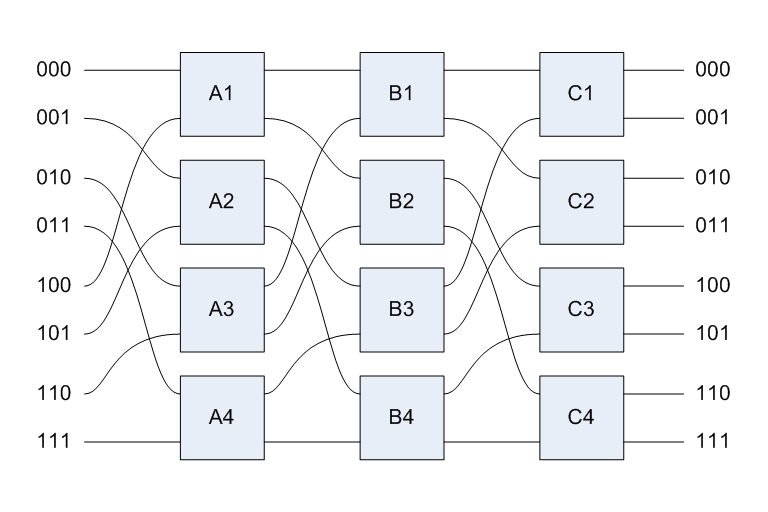
\includegraphics[width = \textwidth]{includes/graphics/OmegaNetwork.jpg}
    By Bjmyers17, CC BY-SA 3.0, \url{https://commons.wikimedia.org/w/index.php?curid=75639225}
\end{defi}

\begin{defi}{Benes-Netzwerk}
    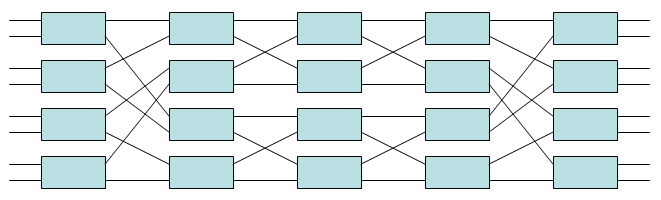
\includegraphics[width = \textwidth]{includes/graphics/Benesnetwork.png}
    By Piggly - Own work, Public Domain, \url{https://commons.wikimedia.org/w/index.php?curid=2988080}
\end{defi}

\subsubsection{Cluster-Interconnects}

\begin{defi}{Cluster-Interconnect}
    
\end{defi}

\begin{defi}{Infiniband}
    \begin{itemize}
        \item \ldots ist eine Architektur für Hochgeschwindigkeitsverbindungen zwischen Rechnern und externen Speicherservern.
        \item \ldots wurde unter Führung von Intel entwickelt, später Mellanox, jetzt Nvidia.
        \item \ldots eignet sich auch als Verbindungsnetzwerk von Rechen-Clustern.
    \end{itemize}
    aktuell: Infiniband EDR / HDR mit bis zu 200 Gbit/s
\end{defi}

\begin{defi}{Gigabit Ethernet}
    \begin{itemize}
        \item \ldots wird vorwiegend in lokalen Netzwerken genutzt,
              auch für Heimanwender mit RJ45 Stecker für Kupferkabel (z.B. Lan-Buchsen am Router)
        \item \ldots ist für Glasfaser und (twisted-pair) Kupferkabel spezifiziert,
              höhrere Bandbreiten aber nur über Glasfaser umsetzbar: bis zu 100 Gb/s
        \item \ldots ist Switch-basiert und abwärtskompatibel
        \item \ldots nutzt spezielle Kollisionserkennung / -vermeidung,
              wie CSMA / CD (Carrier Sense Multiple Access with Collision Detection)
    \end{itemize}
\end{defi}

\begin{defi}[Verbindungsnetzwerk]{Klassifikation}
    \begin{itemize}
        \item Statisch
              \begin{itemize}
                  \item Ein-dimensional
                  \item Zwei-dimensional
                  \item Mehr-dimensional
              \end{itemize}
        \item Dynamisch
              \begin{itemize}
                  \item Bussysteme
                  \item Zellenbasierte Netze
                        \begin{itemize}
                            \item Einstufig
                            \item Mehrstufig
                                  \begin{itemize}
                                      \item Blockierend
                                      \item Nicht-Blockierend
                                  \end{itemize}
                        \end{itemize}
                  \item Kreuzschienenverteiler (Crossbars)
              \end{itemize}
    \end{itemize}
\end{defi}


\include{includes/07_cache.tex}
% \include{includes/08_mehrprozessorsysteme.tex}
% \include{includes/09_multithreading.tex}
% \include{includes/10_vektorrechner.tex}

\printindex
\printindex[Beispiele]

%\printbibliography
\end{document}
